\documentclass[a4paper,12pt,twoside]{article}

%===========PACOTES
\usepackage[body={165mm,235mm}]{geometry}
%\usepackage[portuguese]{babel}
\usepackage{a1}
\usepackage[english]{babel}
\usepackage[latin1]{inputenc} %permite o uso de acentos
%\usepackage[dvips]{color}
\usepackage{amsfonts,amssymb}
%\usepackage{epsfig}
\usepackage{amsmath}
\usepackage{graphicx}	

% makeidx
\usepackage{makeidx}
% make index
\makeindex
%\usepackage[pdftex]{graphicx}


\def\mapright#1#2#3{\smash{\mathop{\hbox to
#3{\rightarrowfill}}\limits^{#1}_{#2}}}

\def\mapleft#1#2#3{\smash{\mathop{\hbox to
#3{\leftarrowfill}}\limits^{#1}_{#2}}}

\def\mapright#1#2{\smash{\mathop{\hbox to 0.90cm{\rightarrowfill}}\limits^{#1}_{#2}}}
\def\mapleft#1#2{\smash{\mathop{\hbox to 0.90cm{\leftarrowfill}}\limits^{#1}_{#2}}}

\def\mapleftright#1#2{\smash{\mathop{\hbox to 0.80cm{\leftarrowfill \rightarrowfill}}\limits^{#1}_{#2}}}
\def\ext{\times \! \vrule depth0pt height5pt width0.35pt}

\def\H{\mathcal H}
\def\D{\mathcal D}
\def\B{\mathcal B}
\def\C{\mathbb C}
\def\R{\mathbb R}
\def\S{\mathbb S}
\def\U{\mathcal U}
\def\Z{\mathbb Z}

\title{A tougher challenge to 3-manifold topologists and group algebraists
\footnote{2010 Mathematics Subject Classification: 
57M25 and 57Q15 (primary), 57M27 and 57M15 (secondary)}} 
\author{S�stenes L. Lins}

\date{\today}


\begin{document}


\maketitle

\begin{abstract}
This paper poses some basic questions about instances (hard to find) of 
a special problem in 3-manifold topology.
``Important though the general concepts and propositions may be with the 
modern industrious passion
for axiomatizing and generalizing has presented us \ldots nevertheless I am convinced that
the special problems in all their complexity constitute the stock and the core of mathematics; 
and to master their difficulty requires on the whole the harder labor.'' Hermann Weyl 1885-1955, 
cited in the preface of the first edition (1939) of A. N. Whitehead's book
{\em The classical groups: their invariants and representations} \cite{whitehead1997}.

In this paper I focus on new uncertainties left unanswered in L. Lins thesis \cite{lins2007blink}
on the homemorphism problem of eleven concrete pairs of closed orientable 3-manifolds induced
by 3-connected monochromatic {\em blinks} (\cite{kauffman1994tlr}). The eleven HG8QI-classes are the 
only doubts left in the thesis, but first two of the eleven were solved few days ago and 
I report on the solution.


\end{abstract}


\section{Introduction}
In a joint recent paper posted recently in the arXiv (\cite{linslinschallenge2013}) 
my son Lauro Lins and me ask some 6 years old questions for which we had no answers
about homeomorphisms between closed orientable 3-manifolds. The two pairs of 3-manifolds
were the only uncertainties that were left in L. Lins thesis  
(\cite{lins2007blink}) under my supervision in the 
domain of 3-manifolds being induced by blackboard framed links (for short {\em bfl}'s) 
up to 9 crossings (9-small 3-manifolds).
A subset of relevant 10-crossings bfl's were generated but their topological classification remains untouched.
The paper was taken seriously by a few researchers, among them M. Culler, N. Dunfield and C. Hodgson 
and others that could solve them very quickly using GAP, SnapPy, Sage, tools that were unknown to us. 
The solutions were obtained by distinct methods and are all consistent (inclusive with BLINK, 
the program of L. Lins (implementing my theory described in \cite{lins1995gca}), which support his thesis). Together
with my colleague Cristiana Nascimento, here at CIn/UFPE, I am learning fast to operate these wonderful tools.
The solutions people found shows that BLINK does a complete job in
topologically classifying the 9-small 3-manifolds.


The first solution that I got, and that blew my mind,  
was by Craig Hodgson using length spectra techniques, based in his
joint paper with J. Weeks entitled {\em Symmetries, 
isometries and length spectra of closed hyperbolic three-manifolds} 
(\cite{hodgson1994symmetries}). By using SnapPy Craig showed that even though the 
quantum WRT-invariants as well as the volumes of the 
hyperbolic $Z$-homology spheres induced by the bfl's),
$U[1466]$ and $U[1563]$ are the same, the length of the 
smallest geodesics of them are distinct. For the other pair of bfl's $U[2125]$ and $U[2165]$ he shows that 
precisely the same facts apply. Here is a summary of Craig's findings extracted from the SnapPy session
that he kindly sent me:\\
\begin{center}
\center{Class $9_{126}$:}
\begin{verbatim}
From first geodesic of U[1466]: 1.0152103824828331+0.39992347315914334j.
From first geodesic of U[1563]: 0.9359206605025168+2.333526236965665j.
Volume of both manifolds: 7.36429600733.
\end{verbatim}
\center{Class $9_{199}$:}
\begin{verbatim}
From first geodesic of U[2125]:  0.8939075859248593+0.761197185679321j.
From first geodesic of U[2165]:  0.7978548001747316+2.9487425029345973j.
Volume of both manifolds: 7.12868652133
\end{verbatim}
\end{center}

 

There were 3 previous versions of \cite{linslinschallenge2013} that I appeared before,
because of annoying mistakes in the presentations and in focusing the challenge in a broader context.
By the way, the presentations are redundant because the blink is enough to define the 3-manifold.
The time spanned between the first (April 22, 2013) and the last version (May 1, 2013) 
was a little more than one week. 
Even so, some people
including Nathan Dunfield worked with the wrong presentations. Not without reason he was angry at me,
but I think that this is no longer true, since he was willing to answer my sometime naive and stupid 
questions and send me a solution for the first pair of manifolds of the present work, 
using Sage and GAP computations, by working with covers. I did not know these tools. Also 
I did not know that the blog on lower dimensional topology
was very active exposing my incorrections and I apologize for my ignorance. 
I thank Cristiana for having calling the blog to my attention.
But I learn fast and do believe that I have something important and different to say in this brave new world of
3-manifolds... After all I have been putting a great amount of time and effort during my scientific carreer, 
(as basically as an isolated researcher) on (mainly closed) 3-manifods. I seek no longer to be isolated.

Marc Culler was very helpful in answering questions of me and Cristiana and helping her about issues in the 
downloading and 
installing SnapPy and Sage and GAP in her machine. After the presentation incorrections out of the 
way he produced an independent proof of the distinctveness of $(U[1466, U[1563])$ and of 
$(U[2125, U[2165])$. He also produced instantaneous isomorphic triangulations of the homeomorphic
3-manifolds in the classes $9_{126}$ and $9_{199}$. This fact makes me anxious to compare and timing the 
performances of BLINK and SnapPy regarding finding homeomorphisms of $k$-small 3-manifolds when the 
homeomrphisms exist.

In this paper I put some new challenges (also coming from
\cite{lins2007blink}), that seem harder than the ones considered in the previous paper. The reason I think so
is that going from 9 to 14,15,16 crossings in the links,
numerical problems start appearing concerning finding the Dirichlet domain and, in these cases, finding
isomorphic triangulations might be harder to SnapPy than to BLINK. At any rate I have hundreds of examples
where the performance of these programs in this issue could be compared, if anyone is seriously interested. Currently
BLINK is not documented and one of my objectives is to seek for help in doing it and extend its capability.
BLINK is hosted at Github under the userid {\em laurolins} and is open source code project. Unfortunately him (currently
a researcher at AT\&T) does not have the necessary time to go on with the implementation. But he welcomes and 
is willing to help collaborators in gettig started. 
As for me, I am too old for the energy needed to construct good pieces of software. I intend to act
as one Scientific Supervisor for the deployment and for the discussions the new algorithms algorithms 
to be included in BLINK, but only at the mathematical level. The technological and software engineering
needed I leave to others. 

An example of such new algoriths that we want to include in BLINK is made possible by the theory 
in Ricardo Machado's thesis
under my supervision, defended last March. We got an $O(n^2)$-algorithm for going from a special kind of gem, 
named resoluble gems, to 
a blink inducing the same manifold. This work is available, in still rather sketch form (even the definition of 
resolubility is unecessary complicated), in the three joint papers
posted last year in the arXiv, {\cite {linsmachadoA2012, linsmachadoB2012, linsmachadoC2012}. The algorithm was
implemented in Mathematica, but it needs to be improved and re-implemented in Java or C++. 
We found a rather crude framed link presentation for
the hyperbolic dodecahedral space (Weber-Seifert manifold). As far as I know nobody has found such 
framed link. My interest in it was aroused by J. Weeks in a visit to the Geometry Center in 1994, when he asked me whether
I had such framed link. The link inducing the Weber-Seifert 3-manifold is given by a 9-component link embedded 
into $\mathbb{R}^3$ and having a total of 68 (only) vertices. (It started with more than 600.)
In a fourth paper under preparation we will show 
that every 3-manifold admits a resoluble gem inducing it.

\section{The eleven classes of tough 3-manifolds}
I assume that the reader has with him a copy of the version 4 of previous challenge paper 
(\cite{linslinschallenge2013}) 
and has learned how to read the manifold either from the blink  or
from the blackboard framed link, \cite{kauffman1994tlr}. As for obtaining a presentation
of the fundamental group based on the Wirtinger relators  (\cite{stillwell1993classical}) 
and the Dehn fillings (\cite{rolfsen2003knots})
the two detailed examples given in \cite{linslinschallenge2013} should suffice, if the reader
has not available other pieces of softwares to get the presentation by automatic means. I had not and
this partially explain my incorrections in the presntations of the 3 firts version: is a messy 
time consuming task to be done by hand, very much prone to errors. 

Actually the first two classes are resolved, only remaining the nine final ones.
The complex numbers in polar form which appear at each $m^t_{p}$-class are the common 
quantum WRT-invariants. All except one of the eleven classes are formed by $Z$-homology spheres.
The exception is $16^t_{56}$ which has no torsion but Betti number 1. These facts are indicated 
by the small number in parenthesis (which  gives the homology of the manifold).

\subsection{The $HG8QI_t$ class $14^t_{24}$:}
\begin{figure}[!h]
\begin{center}
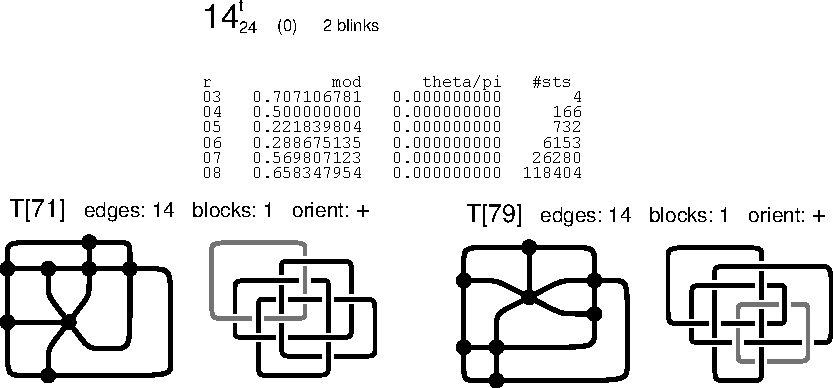
\includegraphics[width=8.2cm]{1.figs/T14_24.pdf}
\caption{\sf The above two manifolds are not homeomorphic. They are distinguished by the homology
of their 5-covers. This was immediately noted by N. Dunfield using Sage and GAP from triangulations
obtained by C. Nascimento using SnapPy, which could not find the Dirichlet domain due to numerical instability. 
}
\label{fig:firstdoubtA}
\end{center}
\end{figure}
\begin{verbatim}
sage: from snappy import *
sage: M1 = Manifold('1424_T71.tri')
sage: M2 = Manifold('1424_T79.tri')
sage: covers1 = M1.covers(5, method='gap')
sage: covers2 = M2.covers(5, method='gap')
sage: [C.homology() for C in covers1]
[Z/132 + Z/132, Z/63 + Z/63, Z/3 + Z/3 + Z/3 + Z/3]
sage: [C.homology() for C in covers2]
[Z/3 + Z/3 + Z/3 + Z/3, Z/213 + Z/213, Z/432 + Z/432]
\end{verbatim}
Above, in verbatim style, is Dunfield's Sage session.
\subsection{The $HG8QI_t$ class $15^t_{16}$:}
\begin{figure}[!h]
\begin{center}
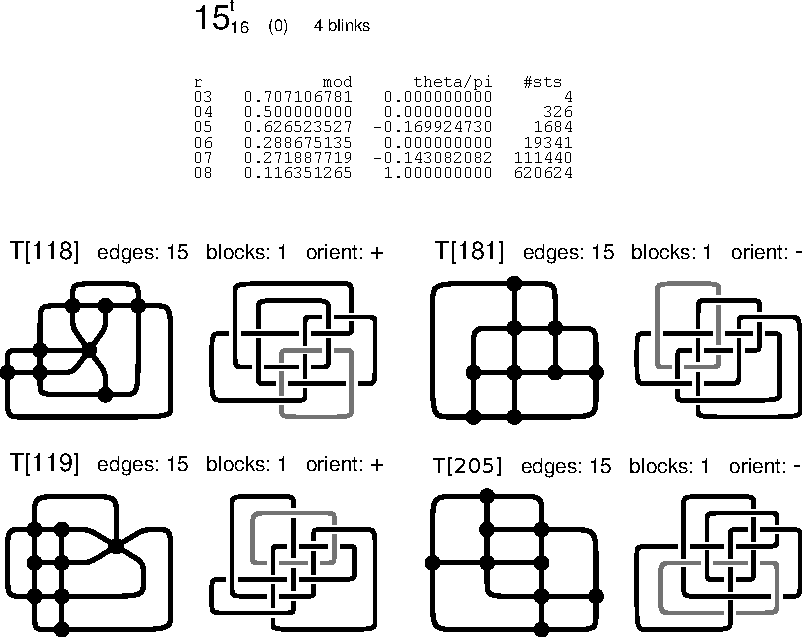
\includegraphics[width=8.2cm]{1.figs/T15_16.pdf}
\caption{\sf The above two manifolds are also non-homeomorphic. 
They are also distinguished by the homology
of their 5-covers. Relative to the class $15^t_{24}$ class $15^t_{16}$
the Sage/GAP software demands much more time.
This was obtained by C. Nascimento using SnapPy/Sage/GAP. The software
SnapPy could not find the Dirichlet domain due to numerical instability. 
}
\label{fig:T15_16}
\end{center}
\end{figure}

\eject
\subsection{The $HG8QI_t$ class $15^t_{19}$:}
\begin{figure}[!h]
\begin{center}
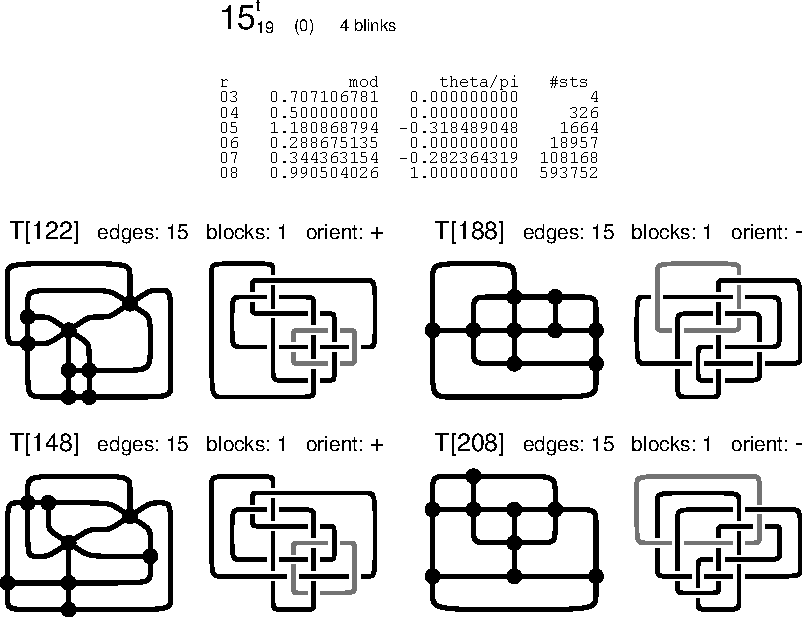
\includegraphics[width=10cm]{1.figs/T15_19.pdf}
\caption{\sf I do not know whether the above four manifolds are homeomorphic or not. 
BLINK says that there are at most two homeomorphisms classes among the four.
}
\label{fig:T15_19}
\end{center}
\end{figure}
\subsection{The $HG8QI_t$ class $15^t_{22}$:}
\begin{figure}[!h]
\begin{center}
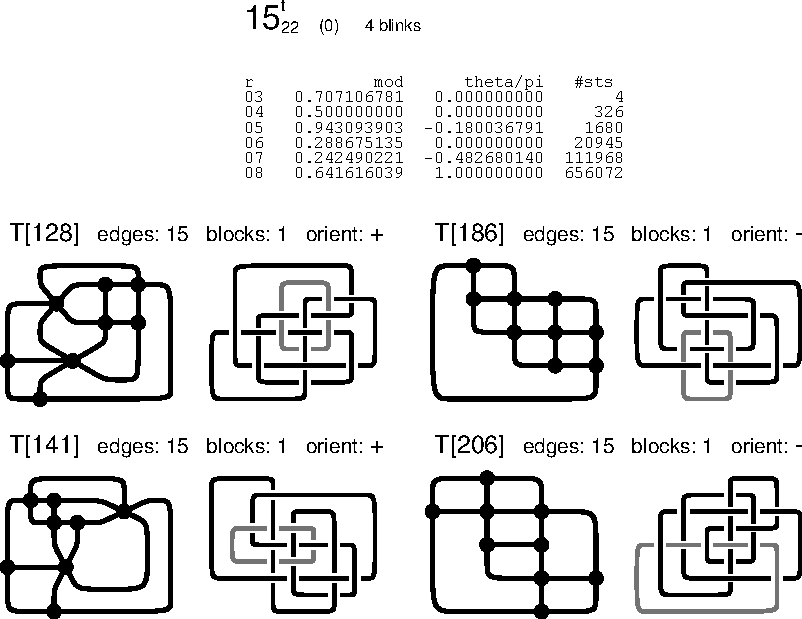
\includegraphics[width=10cm]{1.figs/T15_22.pdf}
\caption{\sf I do not know whether the above four manifolds are homeomorphic or not. 
BLINK says that there are at most two homeomorphisms classes among the four.}
\label{fig:T15_22}
\end{center}
\end{figure}


\eject
\subsection{The $HG8QI_t$ class $16^t_{42}$:}
\begin{figure}[!h]
\begin{center}
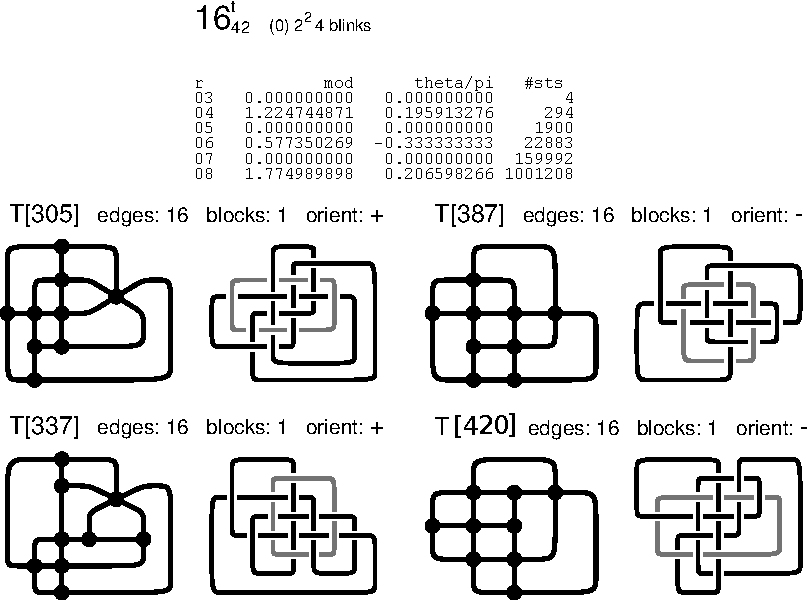
\includegraphics[width=10cm]{1.figs/T16_42.pdf}
\caption{\sf I do not know whether the above four manifolds are homeomorphic or not. 
BLINK says that there are at most two homeomorphisms classes among the four.}
\label{fig:T16_42}
\end{center}
\end{figure}
\subsection{The $HG8QI_t$ class $16^t_{56}$:}
\begin{figure}[!h]
\begin{center}
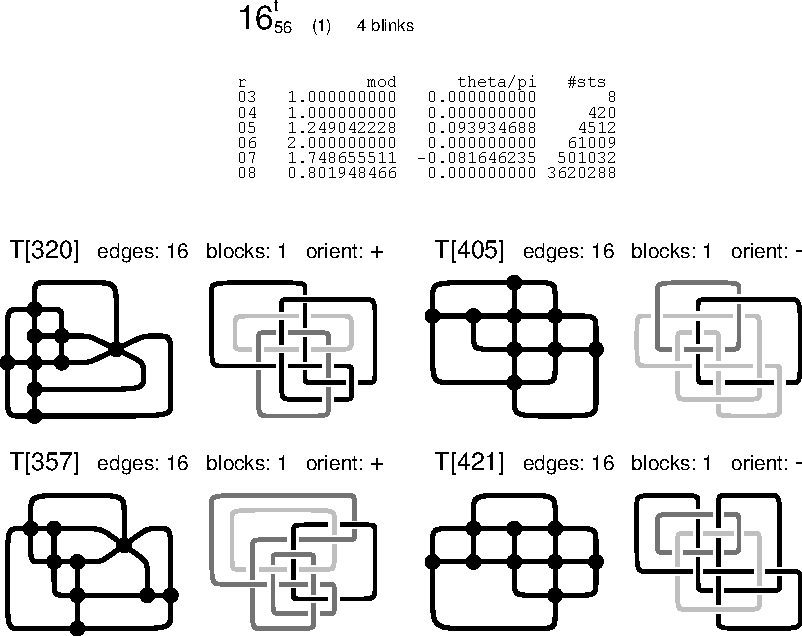
\includegraphics[width=10cm]{1.figs/T16_56.pdf}
\caption{\sf I do not know whether the above four manifolds are homeomorphic or not. 
BLINK says that there are at most two homeomorphisms classes among the four.}
\label{fig:T16_56}
\end{center}
\end{figure}

\eject
\subsection{The $HG8QI_t$ class $16^t_{140}$:}
\begin{figure}[!h]
\begin{center}
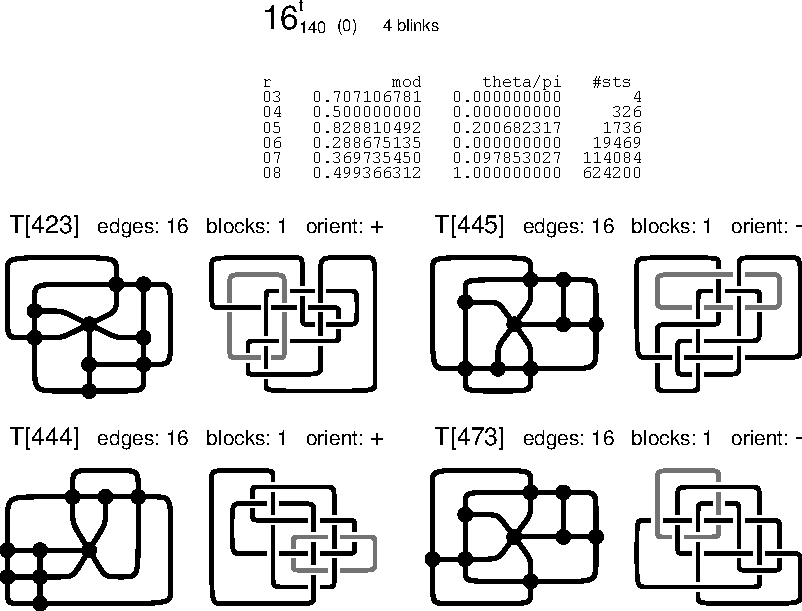
\includegraphics[width=12cm]{1.figs/T16_140.pdf}
\caption{\sf I do not know whether the above four manifolds are homeomorphic or not. 
BLINK says that there are at most two homeomorphisms classes among the four.}
\label{fig:T16_140}
\end{center}
\end{figure}
\subsection{The $HG8QI_t$ class $16^t_{141}$:}
\begin{figure}[!h]
\begin{center}
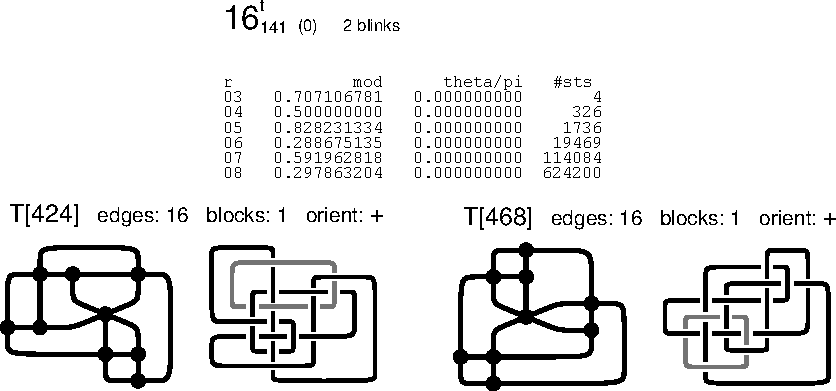
\includegraphics[width=12cm]{1.figs/T16_141.pdf}
\caption{\sf I do not know whether the above two manifolds are homeomorphic or not.}
\label{fig:T16_141}
\end{center}
\end{figure}

\eject
\subsection{The $HG8QI_t$ class $16^t_{142}$:}
\begin{figure}[!h]
\begin{center}
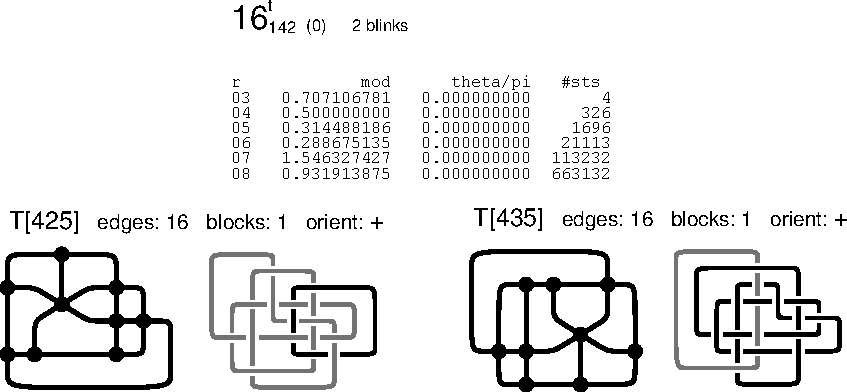
\includegraphics[width=12cm]{1.figs/T16_142.pdf}
\caption{\sf I do not know whether the above two manifolds are homeomorphic or not.}
\label{fig:T16_142}
\end{center}
\end{figure}
\subsection{The $HG8QI_t$ class $16^t_{149}$:}
\begin{figure}[!h]
\begin{center}
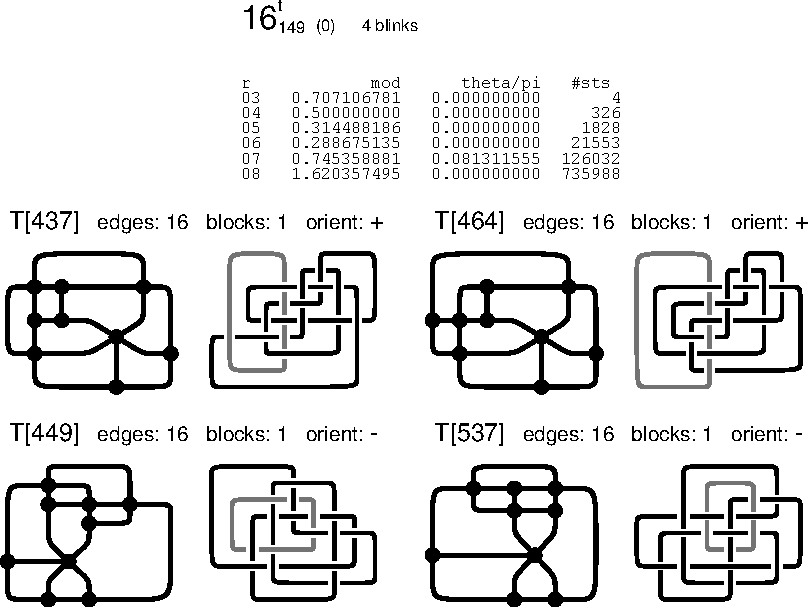
\includegraphics[width=12cm]{1.figs/T16_149.pdf}
\caption{\sf I do not know whether the above four manifolds are homeomorphic or not. 
BLINK says that there are at most two homeomorphisms classes among the four.}
\label{fig:T16_149}
\end{center}
\end{figure}

\eject
\subsection{The $HG8QI_t$ class $16^t_{233}$:}
\begin{figure}[!h]
\begin{center}
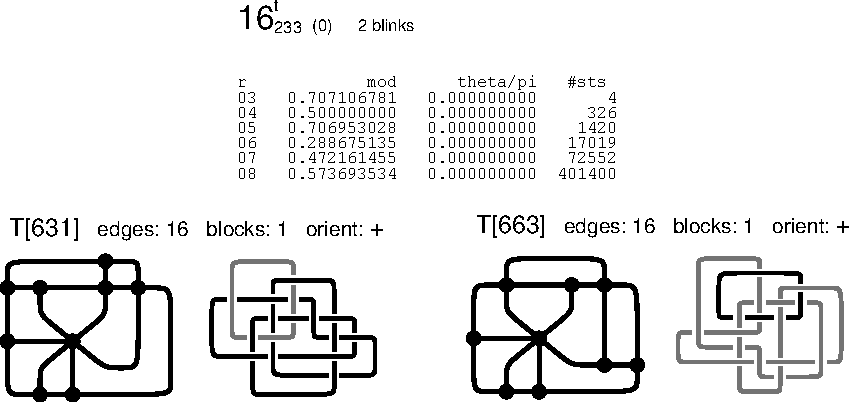
\includegraphics[width=12cm]{1.figs/T16_233.pdf}
\caption{\sf I do not know whether the above two manifolds are homeomorphic or not.}
\label{fig:T16_233}
\end{center}
\end{figure}


\section{Concluding remarks}
The elegant drawings of blinks and blackboard framed links produced by BLINK are 
possible due the groundbreaking algorithm of R. Tamasia \cite{tamassia1987egg}.
Lauro could implement the drawings very fast because we had at hand the implementation of
network flow algorithms he had done for a project to solve {\em practical timetable (!) problems}.
This is an example of the unicity in Mathematics, advocated by L. Lovasz in his famous essay \cite{lovasz1998om}.
To get the drawings one has to apply three times the full strength of network flow theory.
The drawings BLINK presents are in an integer grid and 
deterministically minimize the number of $\pi/2$-bents in the blackboarded framed links.
In particular, it permit us to deal with the unavoidable curls which adjust the integer framings in
the best possible way: we do not care about them. 
The drawings for the companion blinks require a slight modification: it replaces each $p$-valent vertex $p>4$,
by a $p$-polygon inducing 3-valent ones. The final result is massaged a bit to
produce aesthetically pleasing and unambiguous drawings.

As of this writing, C. Hodgson sent me some puzzling 
information (computed with a stronger version of SnapPy) about the first pair of 
manifolds. These are induced by $T[71]$ and $T[79]$, forming the $HG8QI$-class $14_{24}^t$.
They are non-homeomorphic 3-manifolds as first shown by N. Dunfield.
They are homology $\mathbb{Z}$-spheres which have the same WRT-invariants 
(according to BLINK), and quoting Craig {\em ``the same volume (around 24.8) and the same lenght spectra (up to 12 decimals):
the (complex) length of the first geodesic of $T[71]$ is 
0.4749346632398791 + 0i  (of multiplicity 1) 
and that of $T[79]$ is 0.4749346632399361 + 0 i  (of multiplicity 1).''}

\noindent
Here are the Dirichlet domains:
\begin{center}
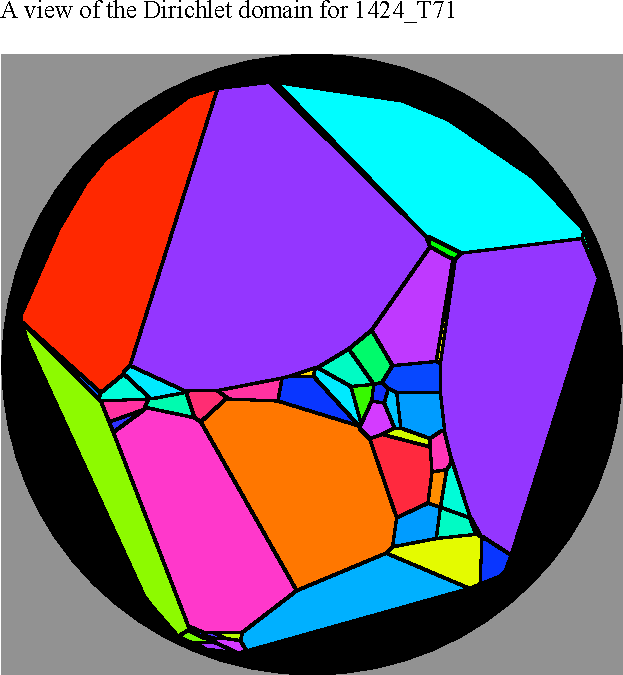
\includegraphics[width=7cm]{1.figs/DirDomT71.pdf}
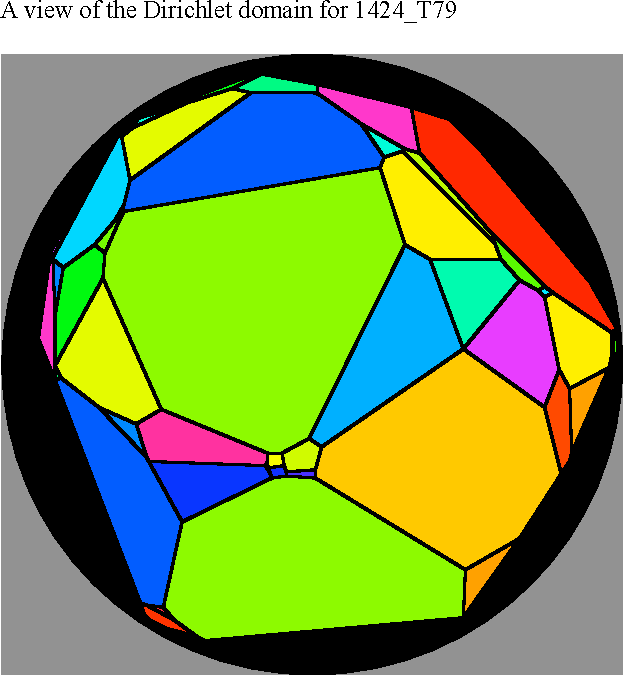
\includegraphics[width=7cm]{1.figs/DirDomT79.pdf}
\end{center}

\noindent
Craig found another proof that $T[71]$ and $T[79]$ are non-homemorphic:
{\em
``Now we can drill out the shortest geodesics using SnapPea to obtain
one-cusped manifolds (the manifold files are attached).
Then SnapPea's isometry checker (which uses the canonical cell decompositions) 
shows that these cusped manifolds are not isometric. Hence the original
closed manifolds are not homeomorphic.
This gives another proof that  $T[71]$ and $T[79]$ are distinct!''}

\noindent
{\bf A final challenge:} 
From the data I could get so far, if a closed orientable 3-manifold is hyperbolic, 
it seems that the WRT-invariants determine its volume. 
Prove it or disproved it.

%-----------------------------------
\bibliographystyle{plain}
%\bibliographystyle{is-alpha}
%\addcontentsline{toc}{bibliografia}{\MakeTextUppercase{Referências Bibliográficas}}
%\bibliography{d:/slsl\3.DadosSostenes.35.ArtigosLivros.bibtexGoogleScholar/bibtexIndex.bib} % bib file is slsl.bib
%\bibliography{~/home/ricardo/Dropbox/35.ArtigosLivros.bibtexGoogleScholar/bibtexIndex.bib}
\bibliography{bibtexIndex.bib}
%\bibliography{slsl}


\vspace{5mm}
\begin{center}
\hspace{7mm}
\begin{tabular}{l}
   S\'ostenes L. Lins\\
   Centro de Inform\'atica, UFPE \\
   Av. Jornalista Anibal Fernandes s/n\\
   Recife, PE 50740-560 \\
   Brazil\\
   sostenes@cin.ufpe.br
\end{tabular}
\end{center}


% \section{Conclusion}
% A closed orientable 3-manifold is denoted {\em $n$-small} if it is induced by surgery on
% a blackboard framed link with at most $n$ crossings.
% Our bet is that both pairs of 3-manifolds in the 2 first sections of 
% this short note are not homeomorphic. This would mean that the $9$-small manifolds are
% completely classified and that
% the combinatorial dynamics of Chapter 4 in \cite{lins1995gca} based 
% on $TS$-moves which leads to a  (small, in the case of hyperbolic 3-manifolds)
% number of minimal gems, named the {\em attractor of
% the 3-manifold} is successful. This induces an efficient algorithm which 
% is capable of classifying topologically all the 3-manifolds given as a blackboard framed link
% with up to (so far) 9 crossings and maintains live the two Conjectures of page 15 of \cite{lins1995gca}:
% the $TS$- and $u^n$-moves yield an efficient algorithm
% to classify $n$-small 3-manifolds by explicitly displaying homeomorphisms, whenever they exist.
% 
% 
% %-----------------------------------
% \bibliographystyle{plain}
% %\bibliographystyle{is-alpha}
% %\addcontentsline{toc}{bibliografia}{\MakeTextUppercase{Refer�ncias Bibliogr�ficas}}
% %\bibliography{d:/slsl\3.DadosSostenes.35.ArtigosLivros.bibtexGoogleScholar/bibtexIndex.bib} % bib file is slsl.bib
% %\bibliography{~/home/ricardo/Dropbox/35.ArtigosLivros.bibtexGoogleScholar/bibtexIndex.bib}
% \bibliography{bibtexIndex.bib}
% %\bibliography{slsl}
% 
% 
% \vspace{5mm}
% \begin{center}
% \hspace{7mm}
% \begin{tabular}{l}
%    S\'ostenes L. Lins\\
%    Centro de Inform\'atica, UFPE \\
%    Av. Jornalista Anibal Fernandes s/n\\
%    Recife, PE 50740-560 \\
%    Brazil\\
%    sostenes@cin.ufpe.br
% \end{tabular}
%\end{center}


\end{document}


